\documentclass{article}

\usepackage[a4paper, total={6in, 9in}]{geometry}

\usepackage{amsmath} % For math
\usepackage{amssymb} % For math
\usepackage{amsthm} % For math
\usepackage{esint} % For math
\usepackage{siunitx} % For SI units

\usepackage{graphicx} % For figures
\usepackage{subcaption} % For figure

\usepackage{float} % For figure placement

\usepackage{minted} % For code

\usepackage{hyperref} % For links
\hypersetup{
	colorlinks,
	citecolor=black,
	filecolor=black,
	linkcolor=black,
	urlcolor=blue,
}
\usepackage{cleveref} % For references

\usepackage{parskip} % For paragraph spacing and no indentation

% \usepackage{tabularx} % For tables
\usepackage[table,xcdraw]{xcolor} % For tables
\def\arraystretch{1.5} % Better looking tables
\usepackage{adjustbox}

% Costum commands:

\newcommand{\qr}{{\quad\Rightarrow\quad}}
\newcommand{\qqr}{{\qquad\Rightarrow\qquad}}



\title{Mandatory 5}
\author{Mathias Balling}
\date{\today}

\begin{document}
\maketitle

\section*{Exercise 4}
Code used for the exercises can be found in "mandatory\_5/", "utils/", and "Numerical-Recipes/".

The equations is set up as follows:
\begin{minted}{cpp}
// V'' = F
double F(double v_prime, double v, double u) {
  return 48 * (pow(v, 3) + 2 * pow(u, 3) * v_prime) *
         (2 * pow(u, 2) - pow(v, 2) * pow(v_prime, 2)) /
         (1 + 64 * pow(u, 6) + 16 * pow(v, 6));
};

// d/dV F = F_v
double F_v(double v_prime, double v, double u) {
  return (48 *
              (3 * pow(v, 2) * (2 * pow(u, 2) - pow(v, 2) * pow(v_prime, 2)) +
               (pow(v, 3) + 2 * pow(u, 3) * v_prime) *
                   (-2 * v * pow(v_prime, 2))) *
              (1 + 64 * pow(u, 6) + 16 * pow(v, 6)) -
          48 * (pow(v, 3) + 2 * pow(u, 3) * v_prime) *
              (2 * pow(u, 2) - pow(v, 2) * pow(v_prime, 2)) *
              (96 * pow(v, 5))) /
         pow(1 + 64 * pow(u, 6) + 16 * pow(v, 6), 2);
};

// d/d(V') F = F_v_prime
double F_v_prime(double v_prime, double v, double u) {
  return 48 *
         (2 * pow(u, 3) * (2 * pow(u, 2) - pow(v, 2) * pow(v_prime, 2)) +
          (pow(v, 3) + 2 * pow(u, 3) * v_prime) * (-2 * pow(v, 2) * v_prime)) /
         (1 + 64 * pow(u, 6) + 16 * pow(v, 6));
};
\end{minted}
\newpage
\subsection*{4.1}
\begin{minted}{text}
|  N   |      A(N)      |     A(N/2)-A(N)    |   alpha^k   |     Rich error      |
|------|----------------|--------------------|-------------|---------------------|
|  2   | -0.86872569807 |                    |             |                     |
|  4   | -0.21646267914 |   -0.652263018932  |             |   0.217421006311    |
|  8   | -0.10093715052 |   -0.115525528625  |  5.6460509  |   0.0385085095417   |
|  16  | -0.52998401181 |   0.429046861297   | -0.2692608  |   -0.143015620432   |
|  32  | -0.50272420575 |   -0.02725980606   | -15.739175  |    0.00908660202    |
|  64  | -0.52565138564 |   0.0229271798843  | -1.1889733  |  -0.00764239329475  |
| 128  | -0.52923104286 |  0.00357965722644  |  6.4048534  |  -0.00119321907548  |
| 256  | -0.52916814457 | -6.28982936317e-05 | -56.911833  |  2.09660978772e-05  |
| 512  | -0.52916397817 |  -4.1663974627e-06 |  15.096565  |  1.38879915423e-06  |
| 1024 | -0.52916368265 |   -2.95528367e-07  |  14.098130  |  9.85094556668e-08  |
\end{minted}
The error is calculated using Richardson extrapolation. For N=1024 the error is $1*10^{-6}$ or better.

The estimate for $V\left(\frac{u_A+u_B}{2}\right)$ is $-0.52916368265$
\subsection*{4.2}
The plot is made using Matplotlib in python: "mandatory\_5/plot.py":

\begin{figure}[H]
  \begin{subfigure}[b]{0.49\textwidth}
    \centering
    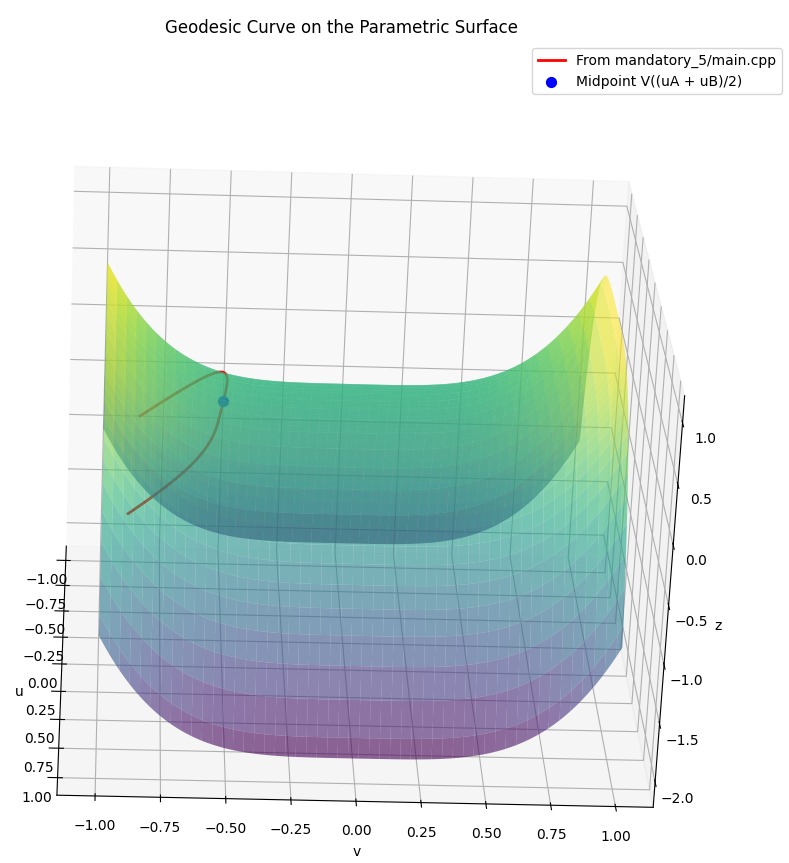
\includegraphics[width=\textwidth]{../plot_front.png}
  \end{subfigure}
  \begin{subfigure}[b]{0.49\textwidth}
    \centering
    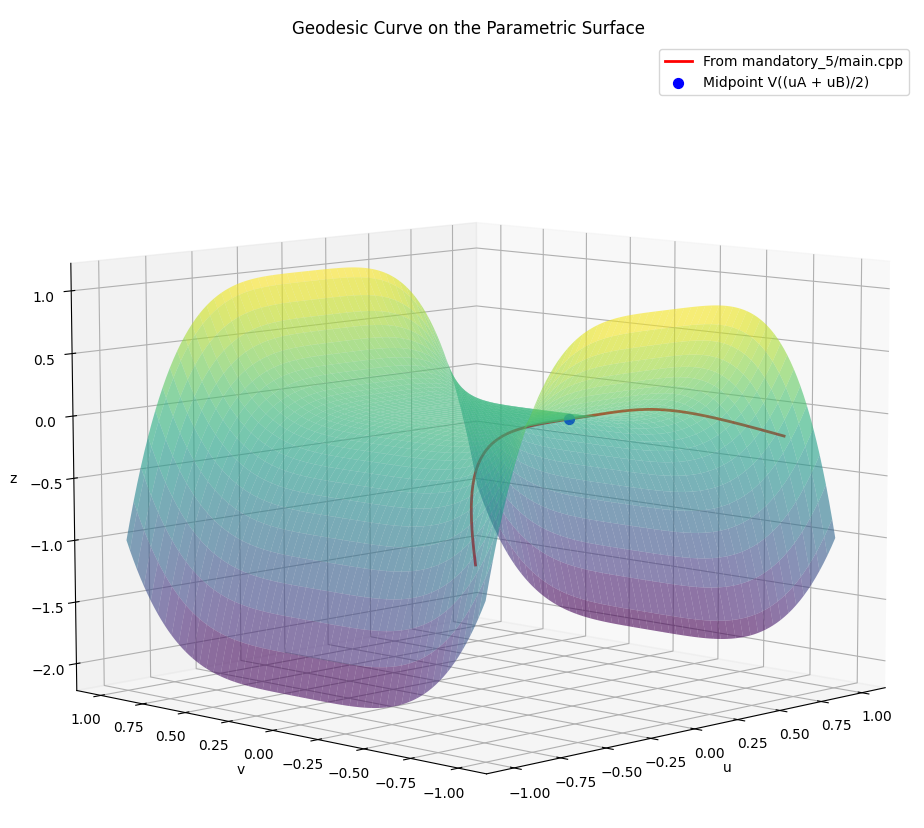
\includegraphics[width=\textwidth]{../plot_side.png}
  \end{subfigure}
\end{figure}

From the plot of the surface with the calculated values overlayed, it seems that they match the curve of the surface. Also the points seems to correctly show the shortest path of the geodesic curve.
\end{document}
